% GNUPLOT: LaTeX picture with Postscript
\begingroup
  \fontfamily{phv}%
  \selectfont
\definecolor{t}{rgb}{0.5,0.5,0.5}
  \makeatletter
  \providecommand\color[2][]{%
    \GenericError{(gnuplot) \space\space\space\@spaces}{%
      Package color not loaded in conjunction with
      terminal option `colourtext'%
    }{See the gnuplot documentation for explanation.%
    }{Either use 'blacktext' in gnuplot or load the package
      color.sty in LaTeX.}%
    \renewcommand\color[2][]{}%
  }%
  \providecommand\includegraphics[2][]{%
    \GenericError{(gnuplot) \space\space\space\@spaces}{%
      Package graphicx or graphics not loaded%
    }{See the gnuplot documentation for explanation.%
    }{The gnuplot epslatex terminal needs graphicx.sty or graphics.sty.}%
    \renewcommand\includegraphics[2][]{}%
  }%
  \providecommand\rotatebox[2]{#2}%
  \@ifundefined{ifGPcolor}{%
    \newif\ifGPcolor
    \GPcolortrue
  }{}%
  \@ifundefined{ifGPblacktext}{%
    \newif\ifGPblacktext
    \GPblacktextfalse
  }{}%
  % define a \g@addto@macro without @ in the name:
  \let\gplgaddtomacro\g@addto@macro
  % define empty templates for all commands taking text:
  \gdef\gplbacktext{}%
  \gdef\gplfronttext{}%
  \makeatother
  \ifGPblacktext
    % no textcolor at all
    \def\colorrgb#1{}%
    \def\colorgray#1{}%
  \else
    % gray or color?
    \ifGPcolor
      \def\colorrgb#1{\color[rgb]{#1}}%
      \def\colorgray#1{\color[gray]{#1}}%
      \expandafter\def\csname LTw\endcsname{\color{white}}%
      \expandafter\def\csname LTb\endcsname{\color{black}}%
      \expandafter\def\csname LTa\endcsname{\color{black}}%
      \expandafter\def\csname LT0\endcsname{\color[rgb]{1,0,0}}%
      \expandafter\def\csname LT1\endcsname{\color[rgb]{0,1,0}}%
      \expandafter\def\csname LT2\endcsname{\color[rgb]{0,0,1}}%
      \expandafter\def\csname LT3\endcsname{\color[rgb]{1,0,1}}%
      \expandafter\def\csname LT4\endcsname{\color[rgb]{0,1,1}}%
      \expandafter\def\csname LT5\endcsname{\color[rgb]{1,1,0}}%
      \expandafter\def\csname LT6\endcsname{\color[rgb]{0,0,0}}%
      \expandafter\def\csname LT7\endcsname{\color[rgb]{1,0.3,0}}%
      \expandafter\def\csname LT8\endcsname{\color[rgb]{0.5,0.5,0.5}}%
    \else
      % gray
      \def\colorrgb#1{\color{black}}%
      \def\colorgray#1{\color[gray]{#1}}%
      \expandafter\def\csname LTw\endcsname{\color{white}}%
      \expandafter\def\csname LTb\endcsname{\color{black}}%
      \expandafter\def\csname LTa\endcsname{\color{black}}%
      \expandafter\def\csname LT0\endcsname{\color{black}}%
      \expandafter\def\csname LT1\endcsname{\color{black}}%
      \expandafter\def\csname LT2\endcsname{\color{black}}%
      \expandafter\def\csname LT3\endcsname{\color{black}}%
      \expandafter\def\csname LT4\endcsname{\color{black}}%
      \expandafter\def\csname LT5\endcsname{\color{black}}%
      \expandafter\def\csname LT6\endcsname{\color{black}}%
      \expandafter\def\csname LT7\endcsname{\color{black}}%
      \expandafter\def\csname LT8\endcsname{\color{black}}%
    \fi
  \fi
  \setlength{\unitlength}{0.0500bp}%
  \begin{picture}(7936.00,5668.00)%
    \gplgaddtomacro\gplbacktext{%
      \csname LTb\endcsname%
      \put(1005,1328){\makebox(0,0){\strut{} 0}}%
      \put(1370,1260){\makebox(0,0){\strut{} 0.1}}%
      \put(1736,1192){\makebox(0,0){\strut{} 0.2}}%
      \put(2101,1124){\makebox(0,0){\strut{} 0.3}}%
      \put(2466,1056){\makebox(0,0){\strut{} 0.4}}%
      \put(2831,988){\makebox(0,0){\strut{} 0.5}}%
      \put(3196,920){\makebox(0,0){\strut{} 0.6}}%
      \put(3561,852){\makebox(0,0){\strut{} 0.7}}%
      \put(3926,784){\makebox(0,0){\strut{} 0.8}}%
      \put(4290,716){\makebox(0,0){\strut{} 0.9}}%
      \put(4655,648){\makebox(0,0){\strut{} 1}}%
      \put(4833,696){\makebox(0,0){\strut{} 0}}%
      \put(5043,814){\makebox(0,0){\strut{} 0.1}}%
      \put(5254,932){\makebox(0,0){\strut{} 0.2}}%
      \put(5465,1050){\makebox(0,0){\strut{} 0.3}}%
      \put(5676,1168){\makebox(0,0){\strut{} 0.4}}%
      \put(5887,1286){\makebox(0,0){\strut{} 0.5}}%
      \put(6097,1404){\makebox(0,0){\strut{} 0.6}}%
      \put(6308,1522){\makebox(0,0){\strut{} 0.7}}%
      \put(6519,1640){\makebox(0,0){\strut{} 0.8}}%
      \put(6730,1758){\makebox(0,0){\strut{} 0.9}}%
      \put(6941,1876){\makebox(0,0){\strut{} 1}}%
      \put(963,2192){\makebox(0,0)[r]{\strut{}-60}}%
      \put(963,2417){\makebox(0,0)[r]{\strut{}-50}}%
      \put(963,2641){\makebox(0,0)[r]{\strut{}-40}}%
      \put(963,2865){\makebox(0,0)[r]{\strut{}-30}}%
      \put(963,3090){\makebox(0,0)[r]{\strut{}-20}}%
      \put(963,3314){\makebox(0,0)[r]{\strut{}-10}}%
      \put(963,3539){\makebox(0,0)[r]{\strut{} 0}}%
      \put(963,3763){\makebox(0,0)[r]{\strut{} 10}}%
      \put(333,2977){\makebox(0,0){\strut{}f(x,y)}}%
      \put(3968,5325){\makebox(0,0){\strut{}Solução numérica para equação de Laplace}}%
    }%
    \gplgaddtomacro\gplfronttext{%
      \csname LTb\endcsname%
      \put(6136,4884){\makebox(0,0)[r]{\strut{}n = 200}}%
      \csname LTb\endcsname%
      \put(2388,771){\makebox(0,0){\strut{}x}}%
      \put(6706,1145){\makebox(0,0){\strut{}y}}%
      \put(333,2977){\makebox(0,0){\strut{}f(x,y)}}%
      \put(7356,2433){\makebox(0,0)[l]{\strut{}-60}}%
      \put(7356,2683){\makebox(0,0)[l]{\strut{}-50}}%
      \put(7356,2934){\makebox(0,0)[l]{\strut{}-40}}%
      \put(7356,3184){\makebox(0,0)[l]{\strut{}-30}}%
      \put(7356,3435){\makebox(0,0)[l]{\strut{}-20}}%
      \put(7356,3685){\makebox(0,0)[l]{\strut{}-10}}%
      \put(7356,3936){\makebox(0,0)[l]{\strut{} 0}}%
      \put(7356,4187){\makebox(0,0)[l]{\strut{} 10}}%
    }%
    \gplbacktext
    \put(0,0){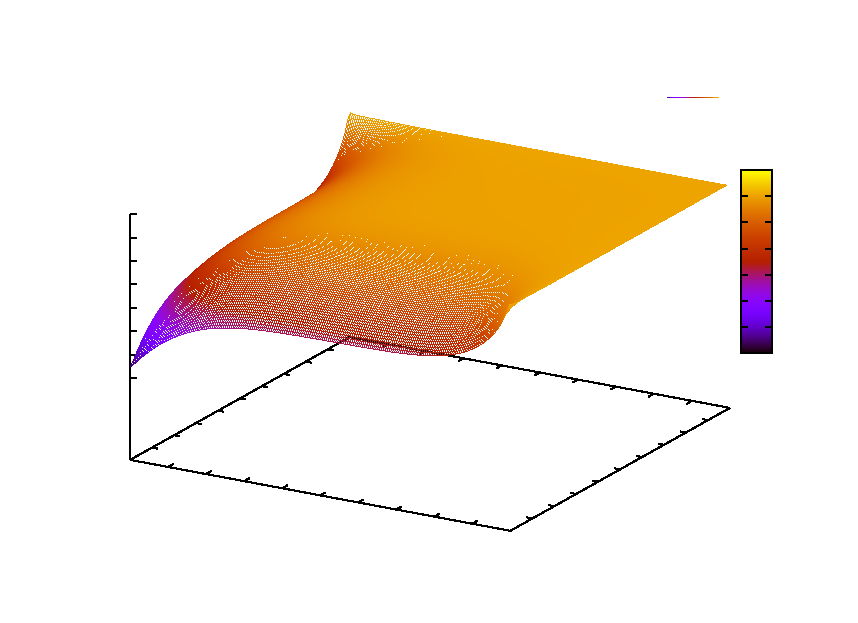
\includegraphics{./graph-01}}%
    \gplfronttext
  \end{picture}%
\endgroup
